%!TEX root=../../main.tex

\chapter{Inference for numerical data}
\label{inferenceForNumericalData}

\begin{comment}
	
	-- Go back to chapter 4 to emphasize the possible use of software to compute normal probabilities.
	
	-- Do the same thing here when discussing computing t probabilities
    
    -- Add two independent group analysis of swim suit data and compare with the correct paired data version
	
\end{comment}


Chapter~\ref{foundationsForInference} introduced some of the primary tools of statistical inference -- point and confidence  interval estimates and hypothesis tests.  This chapter examines some scientific settings where these tools are often used, including the analysis of paired observations and comparing two or more independent groups.  The beginning of the chapter returns to the problem of inference for a population mean, adding a new distribution, the $t$-distribution, which can often be used in small samples. 


%__________________
\section{Inference for one-sample means with the $t$-distribution}
\label{oneSampleMeansWithTDistribution}


The tools studied in Chapter~\ref{foundationsForInference} all made use of the $t$-statistic from a sample mean:
\[
   t = \frac{\overline{x} - \mu}{s}.
\]
The parameter $\mu$ was a population mean, and $\overline{x}$ and $s$ were the sample mean and standard deviation.  Tests and confidence intervals were restricted to samples of at least 30 independent observations from a population where there was no evidence of strong skewness.  This restriction justified appealing to the Central Limit Theorem to calculate probabilities for the $t$-statistic from the normal probability model. If the data are approximately symmetric and there are no large outliers, the $t$-statistic has what is called a $t$-distribution in sample sizes smaller than 30.  That is where the $t-$statistic gets its name.  Using the normal distribution as the sampling distribution of the $t$-statistic essentially treats $s$ as a good replacement for the unknown population standard deviation, $\sigma$.  The sample standard deviation $s$ is really an estimate of $\sigma$, and has an inherent variability just as $\overline{x}$ does.  The $t$ density function has a shape  similar to the normal density but adjusts for the variability in $s$ by having more probability in the left and right tails -- it has more variability.


\subsection{The $t$-distribution}
\label{introducingTheTDistribution}

\index{t-distribution|(}
\index{distribution!$t$|(}

A $t$-distribution, shown as a solid line in Figure~\ref{tDistCompareToNormalDist}, has a bell shape. However, its tails are thicker than the normal model's. This means observations are more likely to fall beyond two standard deviations from the mean than under the normal distribution.\footnote{The standard deviation of the $t$-distribution is actually a little more than 1. However, it is useful to always think of the $t$-distribution as having a standard deviation of 1 in all of our applications.} While our estimate of the standard error will be a little less accurate when we are analyzing a small data set, the extra thick tails of the $t$-distribution correct for the variability in $s$. 

\begin{figure}
\centering
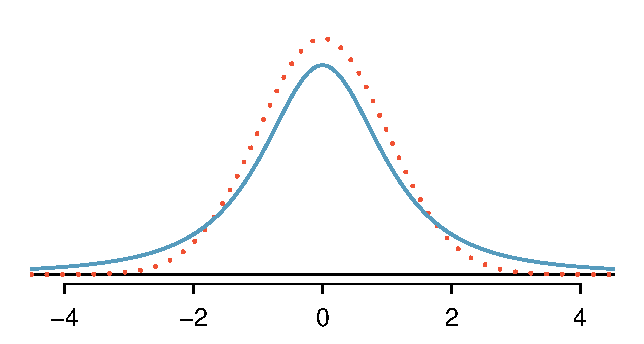
\includegraphics[height=45mm]{ch_inference_for_means_oi_biostat/figures/tDistCompareToNormalDist/tDistCompareToNormalDist}
\caption{Comparison of a $t$-distribution (solid line) and a normal distribution (dotted line).}
\label{tDistCompareToNormalDist}
\end{figure}

The $t$-distribution, always centered at zero, has a single parameter: degrees of freedom.  Several $t$-distributions are shown in Figure~\ref{tDistConvergeToNormalDist}. When there are more degrees of freedom, the $t$-distribution looks very much like the standard normal distribution.

\begin{figure}
\centering
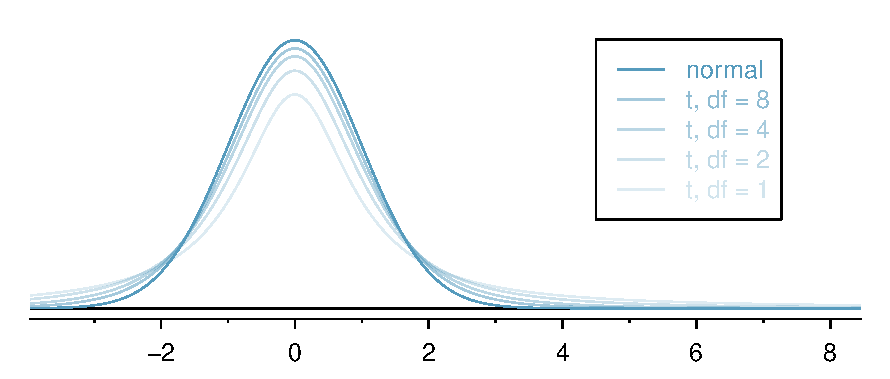
\includegraphics[width=0.8\textwidth]{ch_inference_for_means_oi_biostat/figures/tDistConvergeToNormalDist/tDistConvergeToNormalDist}
\caption{The larger the degrees of freedom, the more closely the $t$-distribution resembles the standard normal model.}
\label{tDistConvergeToNormalDist}
\end{figure}

\begin{termBox}{\tBoxTitle{Degrees of freedom (df)}
The degrees of freedom describe the shape of the $t$-distribution. The larger the degrees of freedom, the more closely the distribution approximates the normal model.}
\end{termBox}

With degrees of freedom of 30 or more, the $t$-distribution is nearly indistinguishable from the normal distribution. The degrees of freedom for the The $t$-statistic in Chapter~\ref{foundationsForInference} has a $t$ distribution with degrees of freedom equal to the sample size - 1, justifying the use of the normal distribution in that chapter.  Section~\ref{tDistSolutionToSEProblem} provides a more complete account of the link between degrees of freedom and sample size.

Probabilities for the $t$-distribution can be calculated using tables of the distribution or using software.  The use of software has become the preferred method because it is more accurate than tables, is not limited to a small range of degrees of freedom and allows complete flexibility in the choice of $t$ values on the horizontal axis.  But each software package uses slightly different commands, so this section illustrates the use of a \term{t-table}, partially shown in Table~\ref{tTableSample}, in place of the normal probability table. A larger $t$-table is in Appendix~\ref{tDistributionTable} on page~\pageref{tDistributionTable}.

\begin{table}[hht]
\centering
\begin{tabular}{r | rrr rr}
one tail & \hspace{1.5mm}  0.100 & \hspace{1.5mm} 0.050 & \hspace{1.5mm} 0.025 & \hspace{1.5mm} 0.010 & \hspace{1.5mm} 0.005  \\
two tails & 0.200 & 0.100 & 0.050 & 0.020 & 0.010 \\
\hline
{$df$} \hfill 1  &  {\normalsize  3.08} & {\normalsize  6.31} & {\normalsize 12.71} & {\normalsize 31.82} & {\normalsize 63.66}  \\ 
2  &  {\normalsize  1.89} & {\normalsize  2.92} & {\normalsize  4.30} & {\normalsize  6.96} & {\normalsize  9.92}  \\ 
3  &  {\normalsize  1.64} & {\normalsize  2.35} & {\normalsize  3.18} & {\normalsize  4.54} & {\normalsize  5.84}  \\ 
$\vdots$ & $\vdots$ &$\vdots$ &$\vdots$ &$\vdots$ & \\
17  &  {\normalsize  1.33} & {\normalsize  1.74} & {\normalsize  2.11} & {\normalsize  2.57} & {\normalsize  2.90}  \\ 
\highlightO{18}  &  \highlightO{\normalsize  1.33} & \highlightO{\normalsize  1.73} & \highlightO{\normalsize  2.10} & \highlightO{\normalsize  2.55} & \highlightO{\normalsize  2.88}  \\ 
19  &  {\normalsize  1.33} & {\normalsize  1.73} & {\normalsize  2.09} & {\normalsize  2.54} & {\normalsize  2.86}  \\ 
20  &  {\normalsize  1.33} & {\normalsize  1.72} & {\normalsize  2.09} & {\normalsize  2.53} & {\normalsize  2.85}  \\ 
$\vdots$ & $\vdots$ &$\vdots$ &$\vdots$ &$\vdots$ & \\
400  &  {\normalsize  1.28} & {\normalsize  1.65} & {\normalsize  1.97} & {\normalsize  2.34} & {\normalsize  2.59}  \\ 
500  &  {\normalsize  1.28} & {\normalsize  1.65} & {\normalsize  1.96} & {\normalsize  2.33} & {\normalsize  2.59}  \\ 
$\infty$  &  {\normalsize  1.28} & {\normalsize  1.64} & {\normalsize  1.96} & {\normalsize  2.33} & {\normalsize  2.58}  \\ 
\end{tabular}
\caption{An abbreviated look at the $t$-table. Each row represents a different $t$-distribution. The columns describe the cutoffs for specific tail areas. The row with $df=18$ has been \highlightO{highlighted}.}
\label{tTableSample}
\end{table}

Each row in the $t$-table represents a $t$-distribution with different degrees of freedom. The columns correspond to tail probabilities. For instance, for a  $t$-distribution with $df=18$, row 18 is used (highlighted in Table~\ref{tTableSample}). The value in this row that identifies the cutoff for an upper tail of 10\% is found in the column where \emph{one tail} is 0.100. This cutoff is 1.33. The the cutoff for the lower 10\% is  -1.33; just like the normal distribution, all $t$-distributions are symmetric.

\begin{example}{What proportion of the $t$-distribution with 18 degrees of freedom falls below -2.10?}
Just like a normal probability problem, we first draw the picture in Figure~\ref{tDistDF18LeftTail2Point10} and shade the area below -2.10. To find this area, we identify the appropriate row: \mbox{$df=18$}. Then we identify the column containing the absolute value of -2.10; it~is the third column. Because we are looking for just one tail, we examine the top line of the table, which shows that a one tail area for a value in the third row corresponds to 0.025. About 2.5\% of the distribution falls below -2.10. In the next example we encounter a case where the exact $t$ value is not listed in the table.
\end{example}

\begin{figure}
\centering
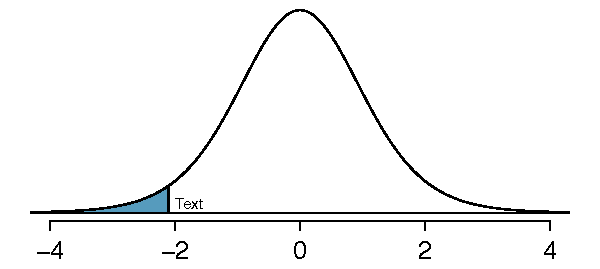
\includegraphics[width=0.5\textwidth]{ch_inference_for_means_oi_biostat/figures/tDistDF18LeftTail2Point10/tDistDF18LeftTail2Point10}
\caption{The $t$-distribution with 18 degrees of freedom. The area below -2.10 has been shaded.}
\label{tDistDF18LeftTail2Point10}
\end{figure}

\begin{example}{A $t$-distribution with 20 degrees of freedom is shown in the left panel of Figure~\ref{tDistDF20RightTail1Point65}. Estimate the proportion of the distribution falling above 1.65.}
We identify the row in the $t$-table using the degrees of freedom: $df=20$. Then we look for 1.65; it is not listed. It falls between the first and second columns. Since these values bound 1.65, their tail areas will bound the tail area corresponding to 1.65. We identify the one tail area of the first and second columns, 0.050 and 0.10, and we conclude that between 5\% and 10\% of the distribution is more than 1.65 standard deviations above the mean. If we like, we can identify the precise area using statistical software: 0.0573.
\end{example}

\begin{figure}
\centering
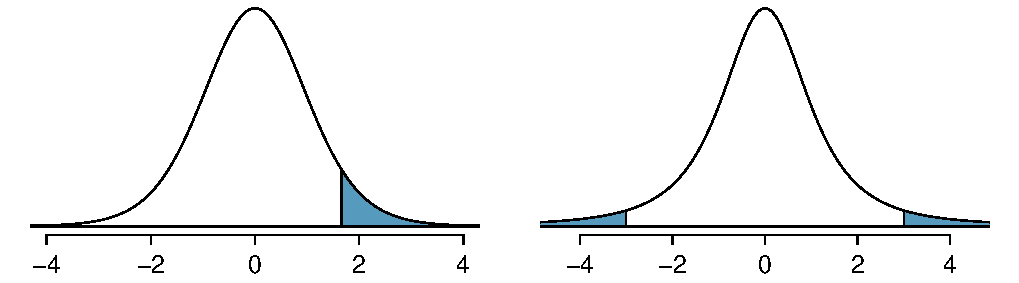
\includegraphics[width=0.85\textwidth]{ch_inference_for_means_oi_biostat/figures/tDistDF20RightTail1Point65/tDistDF20RightTail1Point65}
\caption{Left: The $t$-distribution with 20 degrees of freedom, with the area above 1.65 shaded. Right: The $t$-distribution with 2 degrees of freedom, with the area further than 3 units from 0 shaded.}
\label{tDistDF20RightTail1Point65}
\end{figure}


\subsection{Using the $t$-distribution for tests and confidence intervals for a population mean}
\label{oneSampleTConfidenceIntervalsTests}
\index{data!dolphins and mercury|(}

Chapter~\ref{foundationsForInference} provided formulas for tests and confidence intervals for population means in random samples large enough for the $t$-statistic to have a nearly normal distribution.  In samples smaller than 30 from approximately symmetric distributions without large outliers, the $t$-statistic has a $t$-distribution with degrees of freedom equal to the sample size - 1. Just like inference in larger samples, inference using the $t$-distribution also require that the observations in the sample be independent.  Random samples from very large populations always produce independent observations;  in smaller populations, observations will be approximately independent as long as the size of the sample is no larger than 10\% of the population.

Formulas for tests and intervals using the $t-$distribution are very similar to those using the normal distribution.  For a sample of size $n$ with sample mean $\overline{x}$ and standard deviation $s$, two-sided confidence intervals with confidence coefficient $100(1 - \alpha)$\% have the form
\[
    \overline{x} \pm t_{\text{df}}^{\star}\text{SE},
\]
where 
\begin{itemize}
    
    \item  $\text{SE}= s/\sqrt{n}$ is the standard error of the sample mean;
    
    \item  $t_{\text{df}}^{\star}$ is the point on a $t$-distribution with $n-1$ degrees of freedom and  area $(1 - \alpha/2)$ to its right.
\end{itemize}

A one-sided intervals with the same confidence coefficient will have the form  
\begin{align*}
    \overline{x} &+ t_{\text{df}}^{\star}\text{SE} \text{   (one-sided upper confidence interval)}, \text{  or} \\
    \overline{x} &- t_{\text{df}}^{\star}\text{SE} \text{   (one-sided lower confidence interval)},
\end{align*}
except that in this case $t_{\text{df}}^{\star}$ is the point on a $t$-distribution with $n-1$ degrees of freedom and  area $(1 - \alpha)$ to its right.

\begin{example}{Mercury content in dolphins.}
Dolphins are at the top of the oceanic food chain, which causes dangerous substances such as mercury to concentrate in their organs and muscles. This is an important problem for both dolphins and other animals, like humans, who occasionally eat them. For instance, this is particularly relevant in Japan where school meals have included dolphin at times.
\setlength{\captionwidth}{86mm}

\begin{figure}[h]
\centering
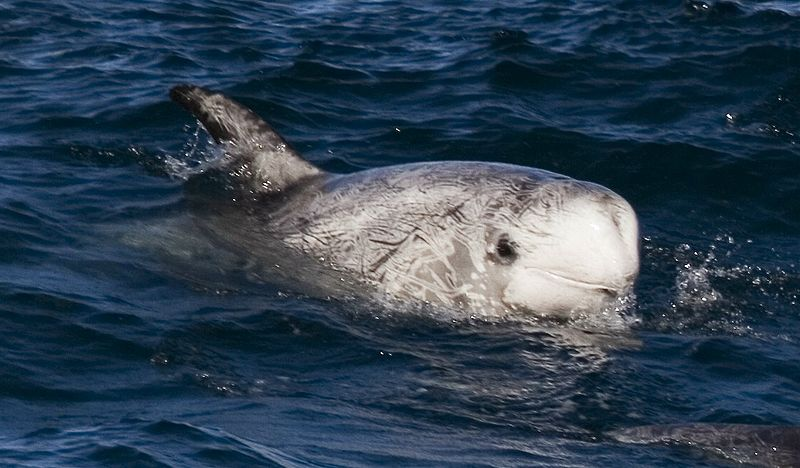
\includegraphics[width=0.8\textwidth]{ch_inference_for_means_oi_biostat/figures/rissosDolphin/rissosDolphin.jpg}  \\
\addvspace{2mm}
\begin{minipage}{\textwidth}
   \caption[rissosDolphinPic]{A Risso's dolphin.\vspace{-1mm} \\
   -----------------------------\vspace{-2mm}\\
   {\footnotesize Photo by Mike Baird (\oiRedirect{textbook-bairdphotos_com}{www.bairdphotos.com}). \oiRedirect{textbook-CC_BY_2}{CC~BY~2.0~license}.}\vspace{-8mm}}
   \label{rissosDolphin}
\end{minipage}
\vspace{3mm}
\end{figure}
\setlength{\captionwidth}{\mycaptionwidth}

This example uses data from a sample of 19 Risso's dolphins from the Taiji area in Japan.\footnote{Taiji was featured in the movie \emph{The Cove}, and it is a significant source of dolphin and whale meat in Japan. Thousands of dolphins pass through the Taiji area annually, and we will assume these 19 dolphins represent a simple random sample from those dolphins. Data reference: Endo T and Haraguchi K. 2009. High mercury levels in hair samples from residents of Taiji, a Japanese whaling town. Marine Pollution Bulletin 60(5):743-747.} The data are summarized in Table~\ref{summaryStatsOfHgInMuscleOfRissosDolphins}. The minimum and maximum observed values can be used to evaluate whether or not there are obvious outliers or skew.

\begin{table}[h]
\centering
\begin{tabular}{ccc cc}
\hline
$n$ & $\overline{x}$ & $s$ & minimum & maximum \\
19   & 4.4	  & 2.3  & 1.7	       & 9.2 \\
\hline
\end{tabular}
\caption{Summary of mercury content in the muscle of 19 Risso's dolphins from the Taiji area. Measurements are in $\mu$g/wet g (micrograms of mercury per wet gram of muscle).}
\label{summaryStatsOfHgInMuscleOfRissosDolphins}
\end{table}

The observations are a simple random sample consisting of less than 10\% of the population, so independence of the observations is reasonable. The summary statistics in Table~\ref{summaryStatsOfHgInMuscleOfRissosDolphins} do not suggest any skew or outliers; all observations are within 2.5 standard deviations of the mean. Based on this evidence, the approximate normality assumption seems reasonable.

With large samples, $z^{\star}$ and the standard error to determine the width of a confidence interval. With a sample size of 19, it will be more accurate to use the $t$-distribution:
\begin{align*}
\overline{x} \pm  t^{\star}_{\text{df}}\text{SE} &= \overline{x}  \pm  t^{\star}_{18} \sqrt{s}/n \\
&= 4.4 \pm  2.10 2.3/\sqrt{19} \\
&= (3.29, 5.51)\,\, \mu\text{g/wet g}.
\end{align*}

The point $z^{\star}$ from a normal distribution is replaced by a point from a $t$-distribution, but sample mean and estimated standard error are unchanged.  In this example the $t^{\star}$ point can be read from the in the $t$-table on page~\pageref{tTableSample}, in the column with area totaling 0.05 in the two tails (third column), the row with 18 degrees of freedom.  Based on these data, one can be 95\% confident the average mercury content of muscles in Risso's dolphins is between 3.29 and 5.51 $\mu$g/wet gram, which is considered high.
\end{example}

The blue fin tuna example in Chapter~\ref{foundationsForInference} cited 0.50 $\mu$g/wet g as the cutoff for safe limits of mercury content.  The two-sided confidence interval for population mean mercury content $
mu$ in the shark muscle example shows that the two-sided hypothesis $H_0: \mu = 0.5$ vs $H_A: \mu > 0.5$ would be rejected at the 0.05 level of significance.  The data provide statistically significant evidence that mercury content in this population is different from 0.1 $\mu$g/wet gram and is, in fact, higher than 0.50.  A formal significance test uses the $t$-statistic
\begin{align*}
	t &= \frac{\overline{x} - \mu_0}{\text{SE}} \\
	  &= \frac{4.4 - 0.50}{2.3/\sqrt{19}} \\
	  &= 7.39.
\end{align*}
Line 18 of the $t$-table on page~\pageref{tTableSample} shows that the probability that the absolute value of a $t$-random variable with 18 df is greater than 7.39 is smaller than 0.01. So for this test, $p < 0.01$, where $p$ is the p-value for the test. Using software, one can show that in fact the $p < 0.001$.

\begin{exercise} \label{croakerWhiteFishPacificExerConditions}
\index{data!white fish and mercury|(}
The FDA's webpage provides some data on mercury content of fish.\footnote{\oiRedirect{textbook-fda_mercury_in_fish_2010}{www.fda.gov/food/foodborneillnesscontaminants/metals/ucm115644.htm}} Based on a sample of 15 croaker white fish (Pacific), a sample mean and standard deviation were computed as 0.287 and 0.069 ppm (parts per million), respectively. The 15 observations ranged from 0.18 to 0.41 ppm. It is reasonable to assume these observations are independent. Based on summary statistics, does the normality assumption seem reasonable? \footnote{There are no obvious outliers; all observations are within 2 standard deviations of the mean. If there is skew, it is not evident. There are no red flags for the normal model based on this (limited) information.}
\end{exercise}

\begin{example}{Estimate the standard error of $\bar{x}=0.287$ ppm using the data summaries in Guided Practice~\ref{croakerWhiteFishPacificExerConditions}. If the $t$-distribution is used to calculte a 90\% confidence interval for the population mean of the mercury content, identify the degrees of freedom and find $t^{\star}_{\text{df}}$.}
\label{croakerWhiteFishPacificExerSEDFTStar}
The standard error: $\text{SE} = \frac{0.069}{\sqrt{15}} = 0.0178$. Degrees of freedom: $\text{df} = n - 1 = 14$.

Using the column where two tails is 0.100 (for a 90\% confidence interval) and row $\text{df}=14$,  $t^{\star}_{14} = 1.76$.
\end{example}

\begin{exercise}
Using the results of Guided Practice~\ref{croakerWhiteFishPacificExerConditions} and Example~\ref{croakerWhiteFishPacificExerSEDFTStar}, compute a 90\% confidence interval for the average mercury content of croaker white fish (Pacific).\footnote{$\bar{x} \ \pm\ t^{\star}_{14} SE \ \to\  0.287 \ \pm\  1.76\times 0.0178\ \to\ (0.256, 0.318)$. We are 90\% confident that the average mercury content of croaker white fish (Pacific) is between 0.256 and 0.318 ppm.}

\index{data!white fish and mercury|)}

\end{exercise}

\section{Paired Data}
\label{pairedData}

\index{paired data|(}


Did a new design for wet suits bring about increased swimming times in the 2000 Olympics? Many people thought so.  de Lucas and co-authors (2000)\footnote{De Lucas et. al, The effects of wetsuits on physiological and biomechanical indices during swimming. \textit{Journal of Science and Medicine in Sport,} 2000; 3(1): 1-8} designed and conducted a study to test the hypothesis that suits had no effect on swimming speed. 

Twelve competitive swimmers swam 1500m at maximum speed, once wearing a wetsuit and once wearing a regular swimsuit, with the order of wetsuit vs swimsuit randomized for each of  the 12 swimmers.  The Investigators recorded maximum velocity for each swimmer, measured in meters per second (m/sec). The data in Table~\ref{swimSuitTimes} can be found in Table 3 the de Lucas paper and in the Lock, et. al. text\footnote{Lock et. al \textit{Statistics, Unlocking the Power of Data}, Wiley, 2013.}

% Tue Jul 26 15:15:14 2016
\begin{table}[ht]
\centering
\begin{tabular}{rrrr}
  \hline
 & swimmer.number & wet.suit.velocity & swim.suit.velocity \\ 
  \hline
1 & 1.00 & 1.57 & 1.49 \\ 
  2 & 2.00 & 1.47 & 1.37 \\ 
  3 & 3.00 & 1.24 & 1.35 \\ 
  4 & 4.00 & 1.35 & 1.27 \\ 
  5 & 5.00 & 1.22 & 1.12 \\ 
  6 & 6.00 & 1.75 & 1.64 \\ 
  7 & 7.00 & 1.64 & 1.59 \\ 
  8 & 8.00 & 1.57 & 1.52 \\ 
  9 & 9.00 & 1.56 & 1.50 \\ 
  10 & 10.00 & 1.53 & 1.45 \\ 
  11 & 11.00 & 1.49 & 1.44 \\ 
  12 & 12.00 & 1.51 & 1.41 \\ 
   \hline
\end{tabular}
\caption{Paired Swim Suit Data} 
\label{swimSuitTimes}
\end{table}

%wet.suit.velocity = c(1.57, 1.47, 1.24, 1.35, 1.22, 
%                      1.75, 1.64, 1.57, 1.56, 1.53, 
%                      1.49, 1.51 )
%swim.suit.velocity = c(1.49, 1.37, 1.35, 1.27, 1.12, 
%                       1.64, 1.59, 1.52, 1.50, 1.45, 
%                       1.44, 1.41)
%swimmer.number = c(1:12)
%swim.suit.study = as.data.frame(cbind(swimmer.number,
%                   wet.suit.velocity, 
%                   swim.suit.velocity))

%swim.suit.study

%xtable(swim.suit.study, caption="Paired Swim Suit Data", 
%       label="swimSuitTimes")
	
The swimsuit velocity dataset is an example of \term{paired data} -- each swimmer has two measured velocities, one with a wet suit and one with a regular swimsuit.  A natural measure of the effect of the wet suit is the difference between the measured maximum velocities (\texttt{diff = wet.suit.veocity - swim.suit.velocity}), and the average difference may shed some light on wet suit effect.  The analysis of the differences from these paired measurements uses the $t$-statistic for a confidence interval and test.  Even though there are two measurements per swimmer, the difference in velocities reduces the problem to a one-sample problem, essentially identical in structure to the problems discussed in Section~\ref{oneSampleMeansWithTDistribution}.

Suppose the parameter $\delta$ is the population average of the difference in maximum velocities during a 1500m swim if all competitive swimmers swam with each swim suit type. This is, of course, a hypothetical population of values, but is useful conceptually in this setting.  When a new intervention is tried for the first time, it is standard practice not to assume that the effect of the intervention will necessarily be positive  -- medicine, for example, has many examples where new drugs thought to be useful turned out to be harmful.  So in this setting, a natural test to start with is the two-sided $t$-test for the hypothesis
\[
    H_0: \delta = 0 \text{  vs.  } H_A: \delta \neq 0.
\]

The important assumptions behind the test which should not be ignored:
\begin{itemize}
	
	\item  The data are a random sample from the population.  The observations are very likely independent, but it is more difficult to justify the assumption that the sample of swimmers is drawn randomly from the population of competitive swimmers.  The swimmers are a collection of volunteers for this study.  Nevertheless, it is often assumed in problems such as this that the swimmers participating in the study are reasonably representative of competitive swimmers.
	
	\item The population of differences is approximately normally distributed.  This is a small sample, one in which normality would be difficult to confirm.  The dot plot for the difference in velocities is shown in Figure~\ref{swimmerDotPlot} and shows approximate symmetry with no large outliers, so the assumption is probably reasonable.
	
\end{itemize}	



\textit{dotplot goes here}

Let $\overline{x}_{\text{diff}}$ denote the sample average of the differences in maximum velocity, $s$ be the standard deviation of the differences, and $n$ the number of pairs in the dataset (12 in this case). The $t$-statistic used to test $H_0$ vs. $H_A$ is 
\[
        \frac{\overline{x}_{\text{diff}} - 0} {s_{\text{diff}}/\sqrt{n}}.
\]
For a general null hypothesis $H_0 = \delta_0$ the $t$ statistic is
\[
        \frac{\overline{x}_{\text{diff}} - \delta_0} {s_{\text{diff}}/\sqrt{n}}.
\]

Here are the steps in testing the hypothesis.

\begin{enumerate}

 \item The null and alternative hypotheses have already been specified.

  \item The choice $\alpha = 0.05$ seems reasonable in this setting.

  \item The $t$-statistic uses the summary mean of the observed differences, $\overline{x}_{\text{diff}} = 0.0625$m/sec, and the standard deviation $s_{\text{diff}} = 0.058$.  The $t$-statistic has value  
\[
	  t = \frac{0.0625 - 0}{0.058/\sqrt{12}} = 3.70. 
\]

\item The two-sided $p$-value is
$$ p = P(T < -\text{3.70}) + P(T > \text{3.70}), $$
where $T$ is a $t$-distributed random variable with $n-1 = 11$  degrees of freedom.
The $t$-table shows that $p < 0.01$. A more accurate value of $p$ (0.004) can be obtained from software. 

\item  The data support the claim that the wet suits changed swim velocity in a 1500 swim. The average increase of 0.0625m/sec is significantly different than  the null hypothesis of no change.

\end{enumerate}

A two-sided 95\% confidence interval for the average velocity difference has the form 
\[ \left(
  \overline{x}_{\text{diff}} - \frac{s_{\text{diff}}}{\sqrt{n}} t^*,
  \:\: \overline{x}_{\text{diff}} + \frac{s_{\text{diff}}}{\sqrt{n}} t^* \right), 
\] 
where $t^*$ is the point on a *t* distribution with $df = n-1 = 11$ that has area 0.025 to its right, 2.20.

The confidence interval has value (0.03, 0.10) m/sec.  Consistent with the results of the hypothesis test, the interval does not include 0 (no change).

The general approach when analyzing paired data is exactly as shown here: calculate the differences between the values in each pair, then use those differences in methods for confidence intervals and tests for a single sample.   Any conclusion from the analysis should be stated in terms of the original paired measurements.


%__________________
\section{Difference of two means}
\label{differenceOfTwoMeans}


Does treatment using embryonic stem cells (ESCs) help improve heart function following a heart attack?  This question, and many like it, are the motivation for studying the effect of interventions in clinical studies. Interventional studies often lead to the comparisons of average outcome in the group with the intervention with the average outcome in the group without the intervention.  Statistically, this is the problem of drawing inference about the difference in two population means, $\mu_1 - \mu_2$, when the data are not paired. The natural statistic is a point estimate of the difference, $\bar{x}_1 - \bar{x}_2$.  This estimate is used to calculate a $t$-statistic that is the basis of confidence intervals and tests.

\subsection{Confidence interval for a difference of means}
\label{confidenceIntervalDifferenceMeans}

\index{data!stem cells, heart function|(}
\index{point estimate!difference of means|(}

Table~\ref{summaryStatsForSheepHeartDataWhoReceivedMiceESCs} contains summary statistics for an experiment to test ESCs in sheep that had a heart attack. Each of these sheep was randomly assigned to the ESC or\text{esc} control group, and the change in their hearts' pumping capacity was measured in the study. A~positive value corresponds to increased pumping capacity, which generally suggests a stronger recovery. This section exhibits a 95\% confidence interval for the effect of ESCs on the change in heart pumping capacity relative to the control group.

The difference in sample means is a point estimate of the difference in outcomes between the two groups:
\begin{eqnarray*}
\bar{x}_{\text{esc}} - \bar{x}_{\text{control}}\ =\ 3.50 - (-4.33)\ =\ 7.83
\end{eqnarray*}

\begin{table}[h]
\centering
\begin{tabular}{l rrrrr}
\hline
\hspace{10mm}	& $n$	& $\bar{x}$	& $s$  	 \\
\hline
ESCs		& 9		& 3.50		& 5.17  	\\
control		& 9		& -4.33		& 2.76  	 \\
\hline
\end{tabular}
\caption{Summary statistics of the embryonic stem cell study.}
\label{summaryStatsForSheepHeartDataWhoReceivedMiceESCs}
\end{table}

%\begin{example}{Set up hypotheses that will be used to test whether there is convincing evidence that ESCs actually increase the amount of blood the heart pumps. Also, check conditions for using the $t$-distribution for inference with the point estimate $\bar{x}_1 - \bar{x}_2$. To assist in this assessment, the data are presented in Figure~\ref{stemCellTherapyForHearts}.}\label{exampleToEvaluteWhetherESCsAreHelpfulInImprovingHeartFunctionInSheep}
%We first setup the hypotheses:
%\begin{itemize}
%\setlength{\itemsep}{0mm}
%\item[$H_0$:] The stem cells do not improve heart pumping function. $\mu_{\text{esc}} - \mu_{\text{control}} = 0$.
%\item[$H_A$:] The stem cells do improve heart pumping function. $\mu_{\text{esc}} - \mu_{\text{control}} > 0$.
%\end{itemize}
%\end{example}

\begin{termBox}{\tBoxTitle{Using the $t$-distribution for a difference in means}
\label{ConditionsForTwoSampleTDist}The $t$-distribution can be used for inference when working with the standardized difference of two means if (1) each sample meets the conditions for using the $t$-distribution and (2) the samples are independent.}
\end{termBox}

\begin{example}{Can the $t$-distribution be used to make inference using the point estimate, $\bar{x}_{\text{esc}} - \bar{x}_{\text{control}} = 7.83$?}
Begin with the two required conditions:
\begin{enumerate}
\item In this study, the sheep were independent of each other. Additionally, the distributions in Figure~\ref{stemCellTherapyForHearts} don't show any prominent outliers, usually an indication in small samples of deviation from normality. This suggests that each sample mean could be modeled using a $t$-distribution.
\item The sheep in each group were also independent of each other.
\end{enumerate}
Because both conditions are met, the $t$-distribution can be used to model the difference of the two sample means.
\end{example}

\begin{figure}[h]
\centering
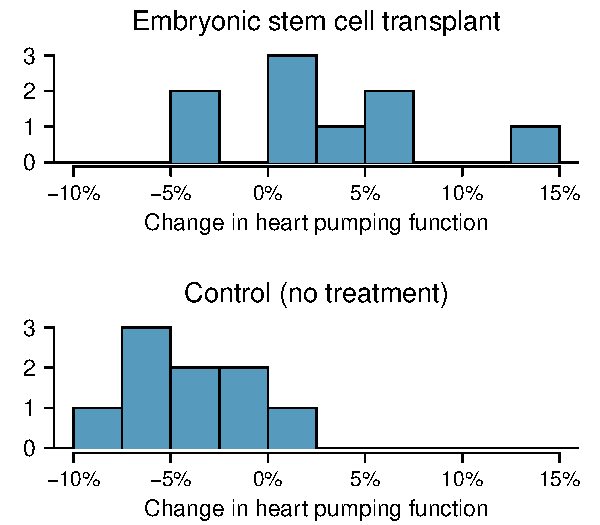
\includegraphics[width=0.58\textwidth]{ch_inference_for_means_oi_biostat/figures/stemCellTherapyForHearts/stemCellTherapyForHearts}
\caption{Histograms for both the embryonic stem cell group and the control group. Higher values are associated with greater improvement. There is no evidence of skew in these data; however, it is worth noting that skew would be difficult to detect with such a small sample.}
\label{stemCellTherapyForHearts}
\end{figure}

%\begin{termBox}{\tBoxTitle{Conditions for applying the $t$-distribution to $\bar{x}_1 - \bar{x}_2$}
%If the sample means, $\bar{x}_1$ and $\bar{x}_2$, each meet the criteria for using the $t$-distribution and the observations in the two samples are independent, then we can analyze the difference in sample means using the $t$-distribution.}
%\end{termBox}

\index{point estimate!difference of means|)}
\index{standard error (SE)!difference in means}

The following formula is used to calculate the standard error of $\bar{x}_{\text{esc}} - \bar{x}_{\text{control}}$:
\index{standard error (SE)!difference in means}
\begin{eqnarray*}
SE_{\bar{x}_{\text{esc}} - \bar{x}_{\text{control}}} = \sqrt{\frac{\sigma_{\text{esc}}^2}{n_{\text{esc}}} + \frac{\sigma_{\text{control}}^2}{n_{\text{control}}}}
\end{eqnarray*}
This standard error is usually estimated using standard deviation estimates from on the samples:
\begin{align*}
SE_{\bar{x}_{\text{esc}} - \bar{x}_{\text{control}}}
	&= \sqrt{\frac{\sigma_{\text{esc}}^2}{n_{\text{esc}}} + \frac{\sigma_{\text{control}}^2}{n_{\text{control}}}} \\
	&\approx \sqrt{\frac{s_{\text{esc}}^2}{n_{\text{esc}}} + \frac{s_{\text{control}}^2}{n_{\text{control}}}}
	= \sqrt{\frac{5.17^2}{9} + \frac{2.76^2}{9}} = 1.95
\end{align*}
The $t$-distribution used in this setting has a somewhat complicated degrees of freedom, usually calculated with software.  An alternative approach uses the smaller of $n_1 - 1$ and $n_2 - 1$, used here in  examples and guided practice.\footnote{This technique for degrees of freedom is conservative with respect to a Type~1 Error; it is more difficult to reject the null hypothesis using this formula for $df$. In this example, computer software would have provided us a more precise degrees of freedom of $\text{df} = 12.225$.}

\begin{termBox}{\tBoxTitle{Distribution of a difference of sample means}
The sample difference of two means, $\bar{x}_1 - \bar{x}_2$, can be modeled using the $t$-distribution and the standard error
\begin{eqnarray}
\textstyle
SE_{\bar{x}_{1} - \bar{x}_{2}} = \sqrt{\frac{s_1^2}{n_1} + \frac{s_2^2}{n_2}}
\label{seOfDifferenceInMeans}
\end{eqnarray}
when each sample mean can itself be modeled using a $t$-distribution and the samples are independent. To calculate the degrees of freedom, use statistical software or the smaller of $n_1 - 1$ and $n_2 - 1$.}
\end{termBox}\textC{\vspace{-10mm}}

\begin{example}{Calculate a 95\% confidence interval for the effect of ESCs on the change in heart pumping capacity of sheep after they've suffered a heart attack.}
The solution uses the sample difference and the its standard error:\textC{\vspace{-3mm}}
\begin{align*}
& \bar{x}_{\text{esc}} - \bar{x}_{\text{control}} = 7.83 \\
& SE = \sqrt{\frac{5.17^2}{9} + \frac{2.76^2}{9}} = 1.95
\end{align*}
With $\text{df} = 8$,  $t^{\star}_{\text{df}} = t^{\star}_{8} = 2.31$ for a 95\% confidence interval:\textC{\vspace{-1mm}}
\begin{align*}
\text{point estimate} \ \pm\ t^{\star}SE \quad\rightarrow\quad
7.83 \ \pm\ 2.31\times 1.95 \quad\rightarrow\quad (3.38, 12.38)
\end{align*}
The data suggest that (with 95\% confidence) embryonic stem cells improve the heart's pumping function in sheep that have suffered a heart attack by 3.38\% to 12.38\%.
\end{example}

\index{data!stem cells, heart function|)}


\subsection{Hypothesis tests for a difference in means}
\label{testingDifferenceMeans}

\index{data!baby\_smoke|(}

The data set \data{baby\_\hspace{0.3mm}smoke} contains a random sample of 150 cases of mothers and their newborns in North Carolina over a year. Four cases from this data set are represented in Table~\ref{babySmokeDF}. This example examines the association between weight if a newborn, \var{weight}, and smoking status of the mother, \var{smoke}.  Does the data contain  evidence that newborns from mothers who smoke have a different average birth weight than newborns from mothers who don't?  The smoking group includes 50 cases and the nonsmoking group contains 100 cases, shown in Figure~\ref{babySmokePlotOfTwoGroupsToExamineSkew}.

\begin{table}[h]
\centering
\begin{tabular}{rrrrrll}
  \hline
 & fAge & mAge & weeks & weight & sexBaby & smoke \\ 
  \hline
1 & NA & 13 &  37 & 5.00 & female & nonsmoker \\ 
  2 & NA & 14 &  36 & 5.88 & female & nonsmoker \\ 
  3 & 19 & 15 &  41 & 8.13 & male & smoker \\ 
  $\vdots$ &   $\vdots$ &   $\vdots$ &   $\vdots$ &   $\vdots$ &   $\vdots$ \\
  150 & 45 & 50 &  36 & 9.25 & female & nonsmoker \\ 
   \hline
\end{tabular}
\caption{Four cases from the \data{baby\_\hspace{0.3mm}smoke} data set. The value ``NA'', shown for the first two entries of the first variable, indicates that piece of data is missing.\textC{-2mm}}
\label{babySmokeDF}
\end{table}

\begin{figure}[hhh]
\centering
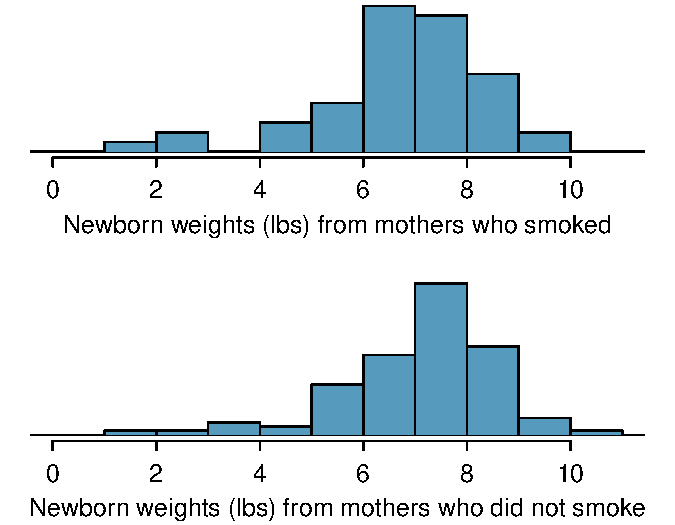
\includegraphics[width=0.63\textwidth]{ch_inference_for_means_oi_biostat/figures/babySmokePlotOfTwoGroupsToExamineSkew/babySmokePlotOfTwoGroupsToExamineSkew}
\caption{The top panel represents birth weights for infants whose mothers smoked. The bottom panel represents the birth weights for infants whose mothers who did not smoke. The distributions exhibit moderate-to-strong and strong~skew, respectively.\index{skew!example: strong}}
\label{babySmokePlotOfTwoGroupsToExamineSkew}
\end{figure}

\begin{example}{Set up appropriate hypotheses to evaluate whether there is a relationship between a mother smoking and average birth weight.}\label{babySmokeHTForWeight}
The null hypothesis represents the case of no difference between the groups.
\begin{itemize}
\setlength{\itemsep}{0mm}
\item[$H_0$:] There is no difference in average birth weight for newborns from mothers who did and did not smoke. In statistical notation: $\mu_{\text{n}} - \mu_{\text{s}} = 0$, where $\mu_{\text{n}}$ represents non-smoking mothers and $\mu_\text{s}$ represents mothers who smoked.
\item[$H_A$:] There is some difference in average newborn weights from mothers who did and did not smoke ($\mu_{\text{n}} - \mu_{\text{s}} \neq 0$).
\end{itemize}
\end{example}

As before, it is important to check the two conditions necessary to apply the $t$-distribution to the difference in sample means. (1) Because the data come from a simple random sample and consist of less than 10\% of all such cases, the observations are independent. Additionally, while each distribution is strongly skewed, the sample sizes of 50 and 100 would make it reasonable to model each mean separately using a $t$-distribution. The skew is reasonable for these sample sizes of 50 and 100. (2) The independence reasoning applied in (1) also ensures the observations in each sample are independent. Since both conditions are satisfied, the difference in sample means may be modeled using a $t$-distribution.

%Summary statistics are shown for each sample in Table~\ref{summaryStatsOfBirthWeightForNewbornsFromSmokingAndNonsmokingMothers}.

\begin{table}[hhh]
\centering
\begin{tabular}{lrr}
	& \resp{smoker} & \resp{nonsmoker} \\
\hline
mean & 6.78 & 7.18 \\
st. dev. & 1.43 & 1.60 \\
samp. size & 50 & 100 \\
\hline
\end{tabular}
\caption{Summary statistics for the \data{baby\_\hspace{0.3mm}smoke} data set.}
\label{summaryStatsOfBirthWeightForNewbornsFromSmokingAndNonsmokingMothers}
\end{table}

\begin{exercise}
The summary statistics in Table~\ref{summaryStatsOfBirthWeightForNewbornsFromSmokingAndNonsmokingMothers} may be useful for this exercise. (a)~What is the point estimate of the population difference, $\mu_{\text{n}} - \mu_{\text{s}}$? (b)~Compute the standard error of the point estimate from part (a).\footnote{(a)~The difference in sample means is an appropriate point estimate: $\bar{x}_{\text{n}} - \bar{x}_{\text{s}} = 0.40$. (b)~The standard error of the estimate can be estimated using Equation~(\ref{seOfDifferenceInMeans}):
\begin{eqnarray*}
SE = \sqrt{\frac{\sigma_n^2}{n_\text{n}} + \frac{\sigma_s^2}{n_\text{s}}}
	\approx \sqrt{\frac{s_n^2}{n_\text{n}} + \frac{s_s^2}{n_\text{s}}}
	= \sqrt{\frac{1.60^2}{100} + \frac{1.43^2}{50}}
	= 0.26
\end{eqnarray*}}
\end{exercise}

\textC{\newpage}

\begin{example}{Draw a picture to represent the $p$-value for the hypothesis test from Example~\ref{babySmokeHTForWeight}.} \label{pictureOfPValueForEstimateOfDiffOfMeansOfBirthWeights}
To depict the $p$-value,  draw the distribution of the point estimate as though $H_0$ were true and shade areas representing at least as much evidence against $H_0$ as what was observed. Both tails are shaded because it is a two-sided test.
\begin{center}
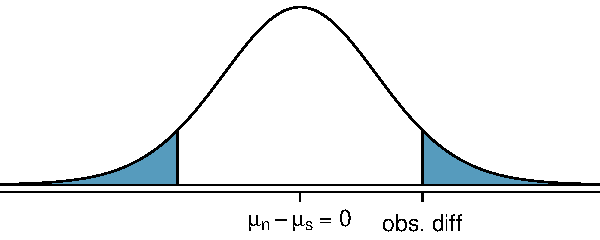
\includegraphics[width=0.6\textwidth]{ch_inference_for_means_oi_biostat/figures/distOfDiffOfSampleMeansForBWOfBabySmokeData/distOfDiffOfSampleMeansForBWOfBabySmokeData}
\end{center}
\end{example}

\begin{example}{Compute the $p$-value of the hypothesis test using the figure in Example~\ref{pictureOfPValueForEstimateOfDiffOfMeansOfBirthWeights}, and evaluate the hypotheses using a significance level of $\alpha=0.05$.} \label{babySmokeHTForWeightComputePValueAndEvalHT}
First compute the T-score:
\begin{eqnarray*}
T = \frac{\ 0.40 - 0\ }{0.26} = 1.54
\end{eqnarray*}
Next, compare this value to values in the $t$-table in Appendix~\vref{tDistributionTable}, using the smaller of $n_{\text{n}} - 1 = 99$ and $n_{\text{s}} - 1 = 49$ as the degrees of freedom: $df = 49$. The T-score falls between the first and second columns in the $df = 49$ row of the $t$-table, so the two-sided $p$-value isbetween 0.10 and 0.20. This p-value is larger than the significance value, 0.05, so the null hypothesis no rejected. There is insufficient evidence to say there is a difference in average birth weight of newborns from North Carolina mothers who did smoke during pregnancy and newborns from North Carolina mothers who did not smoke during pregnancy.
\end{example}

\begin{exercise}
Does the conclusion to Example~\ref{babySmokeHTForWeightComputePValueAndEvalHT} mean that smoking and average birth weight are unrelated?\footnote{No. It is possible that there is some difference but we did not detect it. If there is a difference, we made a Type~2 Error.}
\end{exercise}

\subsection{Pooled standard deviation estimate (special topic)}
\label{pooledStandardDeviations}

Occasionally, two populations will have standard deviations that are so similar that they can be treated as identical. For example, historical data or a well-understood biological mechanism may justify this strong assumption. In such cases, the $t$-distribution approach can be made slightly more precise by using a pooled standard deviation.

The \term{pooled standard deviation} of two groups uses data from both samples to better estimate the common standard deviation and the standard error. If $s_1^{}$ and $s_2^{}$ are the standard deviations of groups 1 and 2 and there are good reasons to believe that the population standard deviations are equal, an improved estimate of the group variances can be obtained by pooling the data from the two groups:
\begin{align*}
s_{\text{pooled}}^2 = \frac{s_1^2 (n_1-1) + s_2^2 (n_2-1)}{n_1 + n_2 - 2}
\end{align*}
where $n_1$ and $n_2$ are the sample sizes, as before. In this setting, the $t$-statistic substitutes $s_{\text{pooled}}^2$ in place of $s_1^2$ and $s_2^2$ in the standard error formula. The degrees of freedom for the $t-$statistic is much simpler in this setting; it is the sum of the degrees of freedom for the two sample variances:
\[
\text{df} = n_1 + n_2 - 2.
\]
The $t$-statistic for testing the hypothesis of no difference between population means becomes 
\[
 t = \frac{\overline{x}_1 - \overline{x}_2}{s_{\text{pooled}}\sqrt{\frac{1}{n_2} + \frac{1}{n_2}}}. 
\]
Significance levels for the statistic are computed using a $t$-distribution with $n_1 + n_2 - 2$ degrees of freedom. The formula for the two-sided confidence interval for the difference in population means is
\[
(\overline{x}_1 - \overline{x}_2) \pm t^{\star} s_p \sqrt{\frac{1}{n_2} + \frac{1}{n_2}},
\]
where $t^{\star}$ is the point on a $t$-distribution with $n_1 + n_2 -2$ degrees of freedom chosen to according the confidence coefficient.

The benefits of pooling the standard deviation are realized through obtaining a better estimate of the standard deviation for each group and using a larger degrees of freedom parameter for the $t$-distribution. Both of these changes may permit a more accurate model of the sampling distribution of $\bar{x}_1 - \bar{x}_2$, if the standard deviations of the two groups are~equal.  In most applications, however, it is difficult to verity th assumption of equal population standard deviations, and it is safer to use the methods discussed in Sections~\ref{confidenceIntervalDifferenceMeans} and \ref{testingDifferenceMeans}.

\begin{caution}
{Pool standard deviations only after careful consideration}
{A pooled standard deviation is only appropriate when background research indicates the population standard deviations are nearly equal. When the sample size is large and the condition may be adequately checked with data, the benefits of pooling the standard deviations greatly diminishes.}
\end{caution}


%__________________
\section[Sample size and power calculations for a difference of means (special topic)]{Power calculations for a difference of means\\ (special topic)}
\label{PowerForDifferenceOfTwoMeans}

The design of a study often involves many complex issues, most of which cannot be covered here.  Perhaps the most important statistical issue in the design stage is choosing an appropriate sample size, and the main aspects of setting a sample size for the comparison of two groups is discussed in this section.  The power of a statistical test is the probability that the test will reject the null hypothesis when the alternative hypothesis is true, so sample sizes are chosen to make that probability sufficiently large, typically between 80 and 90\%.  Power, of course, must be calculated before any data are gathered, since once data and the value of a test statistic are available, it will be clear whether or not the null hypothesis is rejected.

Two competing considerations arise in choosing a sample size:
\begin{itemize}
\setlength{\itemsep}{0mm}
\item The study should be sufficiently large to allow important group differences to be detected in a hypothesis test. 
\item Collecting data is usually expensive and time consuming, and may pose either inconvenience or risk for study subjects.
\end{itemize}
Both issues are particularly important is studies with human subjects.  If an experiment is so small that it is unlikely to find a statistically significant difference even when there are potentially important differences, asking people to participate may waste their time or, even more seriously, expose them to an experimental treatment that might be dangerous.  If a study is larger than needed, more people than necessary will be exposed to an intervention with uncertain value.  It is not an exaggeration to say that studies with human subjects that are either too large or too small are unethical.

This section begins with several subsections that illustrate the concepts in the context of a hypothetical clinical trial, where the goal is to have a sufficient sample size to be 80\% likely to detect practically important effects.\footnote{Similar sample size planning is also important for observational studies, but that is not covered here.}  The last subsection provides formulas that can be used to calculate sample size directly, and mentions software available for doing the calculations.

\subsection{Reviewing the concepts of a test}

\begin{example}{Suppose a pharmaceutical company has developed a new drug for lowering blood pressure, and it is planning a clinical trial to test the drug's effectiveness. The company recruits people who are taking a particular standard blood pressure medication and randomizes the participants either to take a currently accepted medication or to take the new drug.  Participants are usually randomized to one of the two treatments with probability 0.50, and to avoid the bias that might arise if patients or their physician knew the treatment being administered, the pills for both medications are made with identical look and taste. A study is called double-blind when neither physicians nor patients know the treatment received. Write down the hypotheses for a two-sided hypothesis test in this context.}
Generally, clinical trials use a two-sided alternative hypothesis, so below are suitable hypotheses for this context:
\begin{description}
\setlength{\itemsep}{0mm}
\item[$H_0$:] The new drug performs exactly as well as the standard medication. \\
  $\mu_{\text{ \text{trmt}}} - \mu_{\text{ctrl}} = 0$.
\item[$H_A$:] The new drug's performance differs from the standard medication. \\
  $\mu_{\text{ \text{trmt}}} - \mu_{\text{ctrl}} \neq 0$.
\end{description}
Some researchers might argue for a one-sided test here, where the alternative would consider only whether the new drug performs better than the standard medication. However, there are surprisingly many examples where a drug thought to be helpful turns out to produce worse outcomes in a randomized trial. Since it is informative to know whether the new drug performs worse or better than the standard medication, a two-sided test is almost always used in this setting. 
\end{example}

\begin{example}{The company would like to run the clinical trial with participants whose systolic blood pressures are between 140 and 180~mmHg. Suppose previously published studies suggest that the standard deviation of the patients' blood pressures will be about 12~mmHg and the distribution of patient blood pressures will be approximately symmetric.\footnote{In this particular study, measure each participants blood pressure measured at the beginning and end of the study, and the outcome measurement for the study would be the average change in blood pressure in each of the treatment groups. That is, both $\mu_{ \text{trmt}}$ and $\mu_{ \text{ctrl}}$ would represent average differences. Even though the measurement for each participant is a paired difference, the two sets of paired differences (one for each group) are independent measurements from two groups and should be analyzed with a $t$-test for independent groups. The calculations below assume that 12~mmHg is the (unobserved) population standard deviation of a patient's blood pressure difference over the course of the study.} What would be the approximate standard error for $\bar{x}_{ \text{trmt}} - \bar{x}_{ \text{ctrl}}$ if had 100 participants were enrolled in each group?}
The standard error is calculated as follows:
\begin{align*}
SE_{\bar{x}_{ \text{trmt}} - \bar{x}_{ \text{ctrl}}}
  = \sqrt{\frac{s_{ \text{trmt}}^2}{n_{ \text{trmt}}} + \frac{s_{ \text{ctrl}}^2}{n_{ \text{ctrl}}}}
  = \sqrt{\frac{12^2}{100} + \frac{12^2}{100}}
  = 1.70
\end{align*}
This may be an imperfect estimate of $SE_{\bar{x}_{ \text{trmt}} - \bar{x}_{ \text{ctrl}}}$, since the standard deviation estimate we used may not be correct for this group of patients. However, it is sufficient for getting started, and an assumption like this is often all that is available.
\end{example}



% insert OI summary here? or rewrite?



